\documentclass[10pt]{article}
\usepackage[margin=1.0cm]{geometry}
\usepackage[T1]{fontenc}
\usepackage{lmodern}
\usepackage{xcolor}
\usepackage{tikz}
\usepackage{pgfplots}
\usepgfplotslibrary{statistics}
\pgfplotsset{compat=1.18}
\definecolor{srblue}{HTML}{2F6B9A}
\definecolor{opencvorange}{HTML}{D97706}
\definecolor{fps2blue}{HTML}{B9D7EA}
\definecolor{fps5orange}{HTML}{F6C28B}
\definecolor{stslightgreen}{HTML}{A7D8B1}
\definecolor{stsstronggreen}{HTML}{208B3A}
\definecolor{sugarlightpurple}{HTML}{CBB7E8}
\definecolor{sugarstrongpurple}{HTML}{763A9B}
\definecolor{stsedge}{HTML}{1D4E89}
\definecolor{sugaredge}{HTML}{B45309}
\definecolor{incompletegray}{HTML}{9CA3AF}
\definecolor{deltared}{HTML}{B91C1C}
\definecolor{deltagreen}{HTML}{15803D}
\newcommand{\legendcircle}[1]{\tikz[baseline=-0.6ex]\node[draw=black,fill=#1,circle,minimum size=4.5pt,inner sep=0pt] {};}
\newcommand{\legendsquare}[1]{\tikz[baseline=-0.6ex]\node[draw=black,fill=#1,rectangle,minimum size=4.5pt,inner sep=0pt] {};}
\newcommand{\legendtriangle}[1]{\tikz[baseline=-0.6ex]\draw[draw=black,fill=#1,line width=0.4pt] (0,2.3pt)--(-2.3pt,-1.8pt)--(2.3pt,-1.8pt)--cycle;}
\begin{document}
\pagestyle{empty}
\begin{center}
{\Large\bfseries STS-7000: objektmaskierte Bildmetriken}\\[3pt]
{\small Explorative Darstellung; Laufzeit = vollständiger archivierter Pipeline-Lauf}\\[8pt]
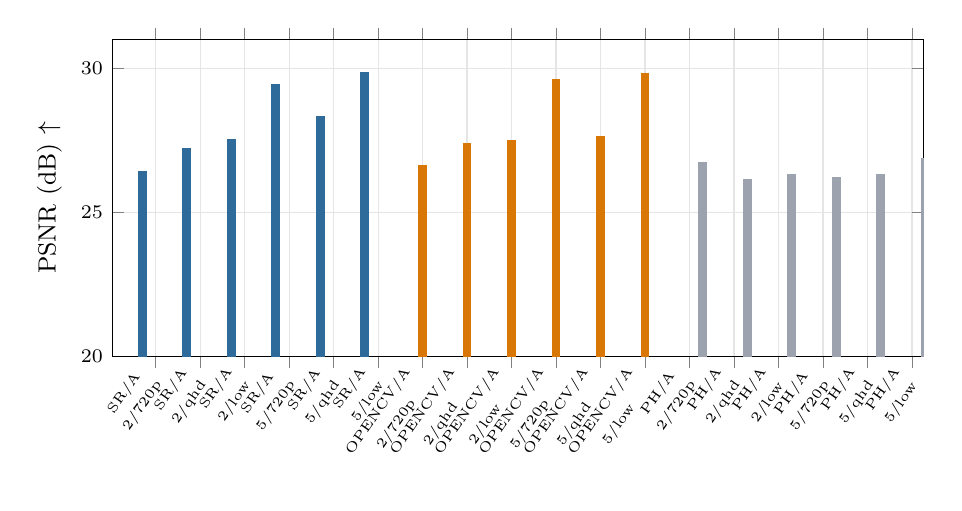
\begin{tikzpicture}
\begin{axis}[height=5.6cm,width=0.98\linewidth,ybar,bar width=2.8pt,enlarge x limits=0.015,xmin=-0.7,ymin=20,ymax=31,xtick=data,xticklabels={{\shortstack{SR/A\\2/720p}},{\shortstack{SR/A\\2/qhd}},{\shortstack{SR/A\\2/low}},{\shortstack{SR/A\\5/720p}},{\shortstack{SR/A\\5/qhd}},{\shortstack{SR/A\\5/low}},{\shortstack{OPENCV/A\\2/720p}},{\shortstack{OPENCV/A\\2/qhd}},{\shortstack{OPENCV/A\\2/low}},{\shortstack{OPENCV/A\\5/720p}},{\shortstack{OPENCV/A\\5/qhd}},{\shortstack{OPENCV/A\\5/low}},{\shortstack{PH/A\\2/720p}},{\shortstack{PH/A\\2/qhd}},{\shortstack{PH/A\\2/low}},{\shortstack{PH/A\\5/720p}},{\shortstack{PH/A\\5/qhd}},{\shortstack{PH/A\\5/low}}},x tick label style={font=\tiny,rotate=55,anchor=east},ylabel style={font=\small},tick label style={font=\scriptsize},ylabel={PSNR (dB) $\uparrow$},grid=major,grid style={gray!20},xtick={0,1,2,3,4,5,6,7,8,9,10,11,12,13,14,15,16,17}]
\addplot+[fill=srblue,draw=srblue] coordinates {(0,26.43472655) (1,27.20227747) (2,27.53329738) (3,29.43136269) (4,28.32448623) (5,29.84945226)};
\addplot+[fill=opencvorange,draw=opencvorange] coordinates {(6,26.63789327) (7,27.40253424) (8,27.50174141) (9,29.62055506) (10,27.63374775) (11,29.83129335)};
\addplot+[fill=incompletegray,draw=incompletegray] coordinates {(12,26.74628133) (13,26.12395680) (14,26.29791524) (15,26.20737476) (16,26.31498760) (17,26.88207464)};
\end{axis}
\end{tikzpicture}
\par\vspace{2pt}
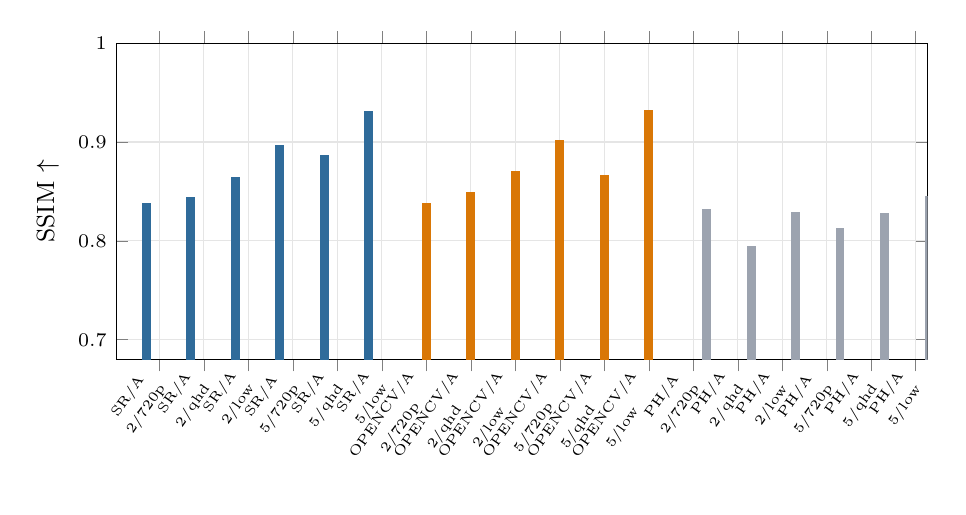
\begin{tikzpicture}
\begin{axis}[height=5.6cm,width=0.98\linewidth,ybar,bar width=2.8pt,enlarge x limits=0.015,xmin=-0.7,ymin=0.68,ymax=1.0,xtick=data,xticklabels={{\shortstack{SR/A\\2/720p}},{\shortstack{SR/A\\2/qhd}},{\shortstack{SR/A\\2/low}},{\shortstack{SR/A\\5/720p}},{\shortstack{SR/A\\5/qhd}},{\shortstack{SR/A\\5/low}},{\shortstack{OPENCV/A\\2/720p}},{\shortstack{OPENCV/A\\2/qhd}},{\shortstack{OPENCV/A\\2/low}},{\shortstack{OPENCV/A\\5/720p}},{\shortstack{OPENCV/A\\5/qhd}},{\shortstack{OPENCV/A\\5/low}},{\shortstack{PH/A\\2/720p}},{\shortstack{PH/A\\2/qhd}},{\shortstack{PH/A\\2/low}},{\shortstack{PH/A\\5/720p}},{\shortstack{PH/A\\5/qhd}},{\shortstack{PH/A\\5/low}}},x tick label style={font=\tiny,rotate=55,anchor=east},ylabel style={font=\small},tick label style={font=\scriptsize},ylabel={SSIM $\uparrow$},grid=major,grid style={gray!20},xtick={0,1,2,3,4,5,6,7,8,9,10,11,12,13,14,15,16,17}]
\addplot+[fill=srblue,draw=srblue] coordinates {(0,0.83750625) (1,0.84375028) (2,0.86402045) (3,0.89666861) (4,0.88654737) (5,0.93094735)};
\addplot+[fill=opencvorange,draw=opencvorange] coordinates {(6,0.83810464) (7,0.84851337) (8,0.87021772) (9,0.90197567) (10,0.86567958) (11,0.93198098)};
\addplot+[fill=incompletegray,draw=incompletegray] coordinates {(12,0.83213003) (13,0.79468482) (14,0.82844450) (15,0.81296965) (16,0.82779669) (17,0.84487853)};
\end{axis}
\end{tikzpicture}
\par\vspace{2pt}
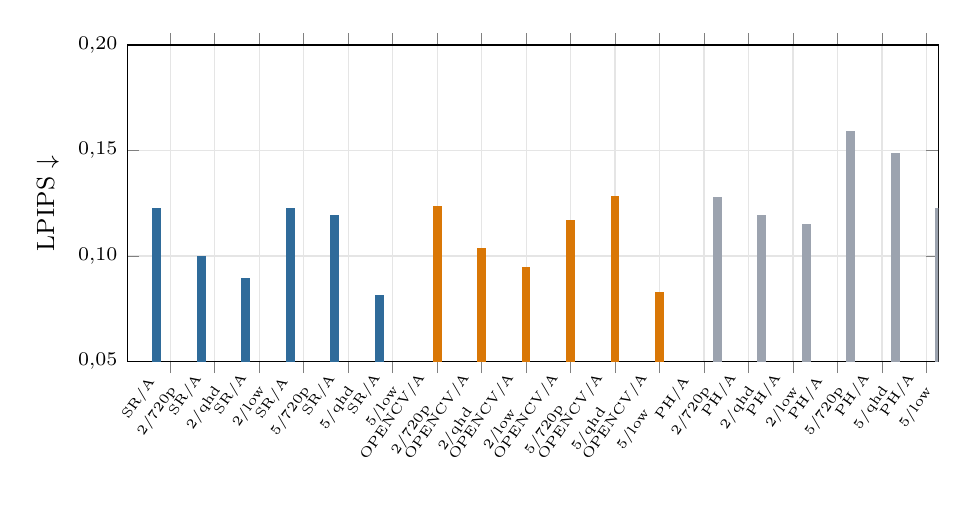
\begin{tikzpicture}
\begin{axis}[height=5.6cm,width=0.98\linewidth,ybar,bar width=2.8pt,enlarge x limits=0.015,xmin=-0.7,ymin=0.05,ymax=0.2,xtick=data,xticklabels={{\shortstack{SR/A\\2/720p}},{\shortstack{SR/A\\2/qhd}},{\shortstack{SR/A\\2/low}},{\shortstack{SR/A\\5/720p}},{\shortstack{SR/A\\5/qhd}},{\shortstack{SR/A\\5/low}},{\shortstack{OPENCV/A\\2/720p}},{\shortstack{OPENCV/A\\2/qhd}},{\shortstack{OPENCV/A\\2/low}},{\shortstack{OPENCV/A\\5/720p}},{\shortstack{OPENCV/A\\5/qhd}},{\shortstack{OPENCV/A\\5/low}},{\shortstack{PH/A\\2/720p}},{\shortstack{PH/A\\2/qhd}},{\shortstack{PH/A\\2/low}},{\shortstack{PH/A\\5/720p}},{\shortstack{PH/A\\5/qhd}},{\shortstack{PH/A\\5/low}}},x tick label style={font=\tiny,rotate=55,anchor=east},ylabel style={font=\small},tick label style={font=\scriptsize},ylabel={LPIPS $\downarrow$},grid=major,grid style={gray!20},scaled y ticks=false,ytick={0.05,0.10,0.15,0.20},yticklabels={{0,05},{0,10},{0,15},{0,20}},xtick={0,1,2,3,4,5,6,7,8,9,10,11,12,13,14,15,16,17}]
\addplot+[fill=srblue,draw=srblue] coordinates {(0,0.12228184) (1,0.09976729) (2,0.08927700) (3,0.12238796) (4,0.11922733) (5,0.08130772)};
\addplot+[fill=opencvorange,draw=opencvorange] coordinates {(6,0.12340123) (7,0.10359985) (8,0.09469956) (9,0.11661723) (10,0.12818055) (11,0.08247017)};
\addplot+[fill=incompletegray,draw=incompletegray] coordinates {(12,0.12784538) (13,0.11916712) (14,0.11490832) (15,0.15874962) (16,0.14865334) (17,0.12247473)};
\end{axis}
\end{tikzpicture}
\par\vspace{2pt}
\vspace{3pt}
\begin{minipage}{0.98\linewidth}\scriptsize Dargestellt werden ausschließlich vollständige Original-GS-A-Routen. Vorhandene \texttt{sts\_masked.json}-Dateien aus später fehlgeschlagenen SuGaR-Routen bleiben als Fehlernachweis archiviert, werden hier aber nicht zusätzlich dargestellt. Die Auswertung ist objektmaskiert; die Werte stammen aus der jeweiligen Runauflösung.\end{minipage}
\end{center}
\end{document}